\section{Technologievergleich}
F\"ur das Projekt soll ein \ac{DMS} verwendet werden, mit welchem sich die vorhandenen Dokumente der \ac{LUBW}, der \ac{GAA} und der \ac{ICT-ENSURE} einfach und bequem in einem System verwalten lassen. Hierbei soll kein \ac{ECM}-Tool vom Grund auf neu entwickelt werden. 

Es soll wie in der Aufgabenstellung im Lastenheft im Kapitel \ref{Lastenheft} festgehalten ein passendes Tool gesucht werden, welches die gegebenen Anforderungen bestm\"oglich erf\"ullt. Die Betrachtung erfolgt hierbei unter der Beachtung g\"angiger Standards.

Das \ac{ECM}-Tool, welches f\"ur das Projekt verwendet werden soll, muss die im folgenden genannten Eigenschaften aufweisen:

\begin{itemize}
 \item Grundlegende Metadatenstandards wie zum Beispiel "`Dublin Core"' und "`EXIF"' m\"ussen unterst\"utzt werden. (siehe Kapitel \ref{Analyse Datenbestaende})
 \item Das System muss alle Fachsysteme der \ac{LUBW} vereinen, welche im Kapitel \ref{Stand der Technik} beschriebenen sind.
 \item Metadaten sollten vom System systematisch gegliedert werden k\"onnen, wie es im Kapitel \ref{Erstellung eines Datenkonzepts} erarbeitet wurde
 \item Das verwendete \ac{ECM}-Tool sollte m\"oglichst viele Schnittstellen bieten, \"uber welche die Daten abgerufen werden
 \item Dateien m\"ussen Versioniert werden k\"onnen um auch \"altere Versionen einsehen zu k\"onnen
 \item Da das Projekt als Prototyp behandelt wird, sollen f\"ur die Umsetzung keine Kosten entstehen
\end{itemize}

Im folgenden werden nun verschiedene namenhafte \ac{ECM}-Tools vorgestellt und auf die eben genannten Eigenschaften gepr\"uft. Am Ende werden die M\"oglichkeiten verglichen und die beste ausgew\"ahlt.


% Damit ein Tool f\"ur dieses Projekt ausgew\"ahlt werden kann, muss es die im folgenden beschriebenen Eigenschaften beinhalten.

% Das Lastenheft im Kapitel \ref{Lastenheft} besagt, dass im Verlauf der Arbeit ein \ac{ECM}-Tool verwendet werden soll,
\subsection{Agorum Core}
Bei "`Agorum Core"' handelt es sich um eine Open Source Software, welche von der Baden W\"urttembergischen Firma "`agorum Software"' stammt. "`Agorum Core"' wird in mehrerem Varianten angeboten. Zum einem gibt es eine freie Version, welche ohne Lizenzkosten genutzt werden kann, zum anderem gibt es mehrere kostenpflichtige Versionen die in ihrem Versionsumfang variieren. \cite{agorum_home} 

Agorum bietet viele Funktionen an, welche jedoch in der freien Version nicht vorhanden sind. Um die zus\"atzlichen Funktionen zu nutzen, muss entweder die ents\"prechende Version, welche die Funktion enth\"alt gekauft werden oder es muss die entsprechende Funktion hinzugebucht werden.
Somit entstehen auf jedenfall Kosten, wenn die freie Version von "`Agorum Core"' nicht die gew\"unschten Funktionen bietet. Weiterhin f\"allt negativ auf, das ein hinzubuchen von Funktionen unter der freien Version nicht m\"oglich ist. \cite{agorum_preise} \cite{Eval_DMS_Bachelor}

In Abbildung \ref{metadatendesigner agorum}\footnote{\url{http://www.agorum.com/uploads/pics/agorum-core-metadatendesigner_01.png}} ist das Web-Interface von "`agorum core"' zu sehen, wobei hier im speziellen der "`Metadaten Designer"' zu sehen ist. Dieses Tool, ist jedoch ein Zusatzfeature, welches entsprechend hinzugebucht werden muss, was nur innerhalb einer "`Pro"'-Version von "`agorum core"' m\"oglich ist. \cite{agorum_metadesigner_bild}

Der "`Metadaten Designer"' kann verwendet werden, um nutzerspezifische Metadatens\"atze zu erstellen.  Da f\"ur die Arbeit keine "`Pro"'-Version von "`agorum core"' gekauft wurde, kann auf die genaue Verwendung leider nicht eingegangen werden. \cite{agorum_metadaten_designer_video}

\begin{figure}[!ht]
\centering
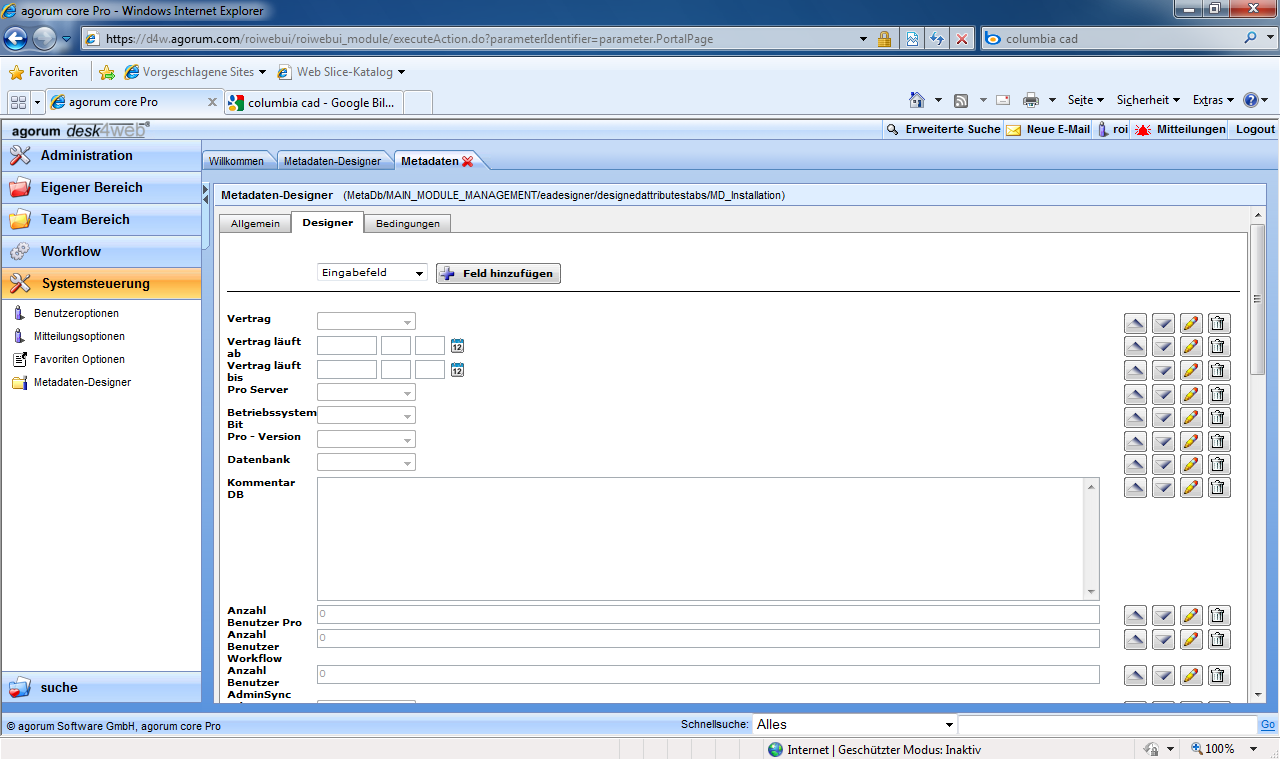
\includegraphics[width=16cm]{Bilder/agorum-core-metadatendesigner.png}
\caption{Metadaten Designer von "`agorum core"' im Web-Interface}
\label{metadatendesigner agorum}
\centering
\end{figure}

Das Einlesen und Bereitstellen von Dokumenten in "`agorum core"' funktioniert schon mit der freien Version. Jedoch kann hier nur eine Standard Suche und Ablage verwendet werden. \cite{agorum_preise}

Das automatische erkennen von Standard-Metadaten in Dateien funktioniert, jedoch auch nur mit der entsprechenden "`Pro"'-Version oder einer Zubuchung genau wie die Versionierung von Dateien.

"`agorum core"' verf\"ugt \"uber verschiedene Schnittstellen, welche von Frontends angesprochen werden k\"onnen. 

\subsection{Alfresco}
Alfresco ist eines der heute am weitesten verbreitete \ac{ECM}-Tool, welches Open Source ist und frei heruntergeladen werden kann.
Flexibilit\"at, Akzeptanz und Skalierbarkeit sind jedoch nur einige der St\"arken, die Alfresco zum Open-Source-Marktf\"uhrer der \ac{ECM}-Branche gemacht haben. \cite{Alfresco_und_Liferay} \cite{Wiki_Alfresco} \cite{Alfresco_Implementation}

Alfresco stammt ebenfalls von einer deutschen Firma, der "`Alfresco Software AG"', und ist somit wie schon agorum auch in deutsch Verf\"ugbar. Namenhafte Unternehmen wie "`Airbus"' oder "`Michelin"' die Software, nach angaben der Herstellers. \cite{Alfresco_Website}

In Abbildung \ref{Alfresco Dashboard} ist das Administrator-Dashboard von Alfresco zu sehen, welches im Webbrowser dargestellt wird.
Im oberen Bildteil ist die Navigationsleiste und das Dash mit m\"oglichen ersten Schritten.

Links ist zum einen das Dash "`Meine Sites"' zu sehen, in welchem alle Seiten zu sehen sind, denen der Nutzer angeh\"ort. Au\ss{}erdem ist darunter ein Dash, welches Aufgaben anzeigt, die vom Benutzer abgearbeitet werden sollen. In Alfresco ist es \"ublich mit Dokumenten und Dateien auch aufgaben zu verkn\"upfen und Workflows zu gestalten. Dies geht f\"ur jede Datei einzeln oder aber auch f\"ur einen Stack von Dateien.

Im Dash, neben "`Meine Sites"' sind die Aktivit\"aten zu sehen, welche zuletzt passiert sind. Hier kann der Nutzer einstellen, in welchen Zeitraum, f\"ur welche Aktivit\"at oder f\"ur welche Elemente er Aktivit\"aten anzeigen lassen m\"ochte.
Darunter ist ein Dash zu sehen, an welchem ein Nutzer sehen kann welche Dokumente er zul\"atzt hochgeladen oder ge\"andert hat.

\begin{figure}[!ht]
\centering
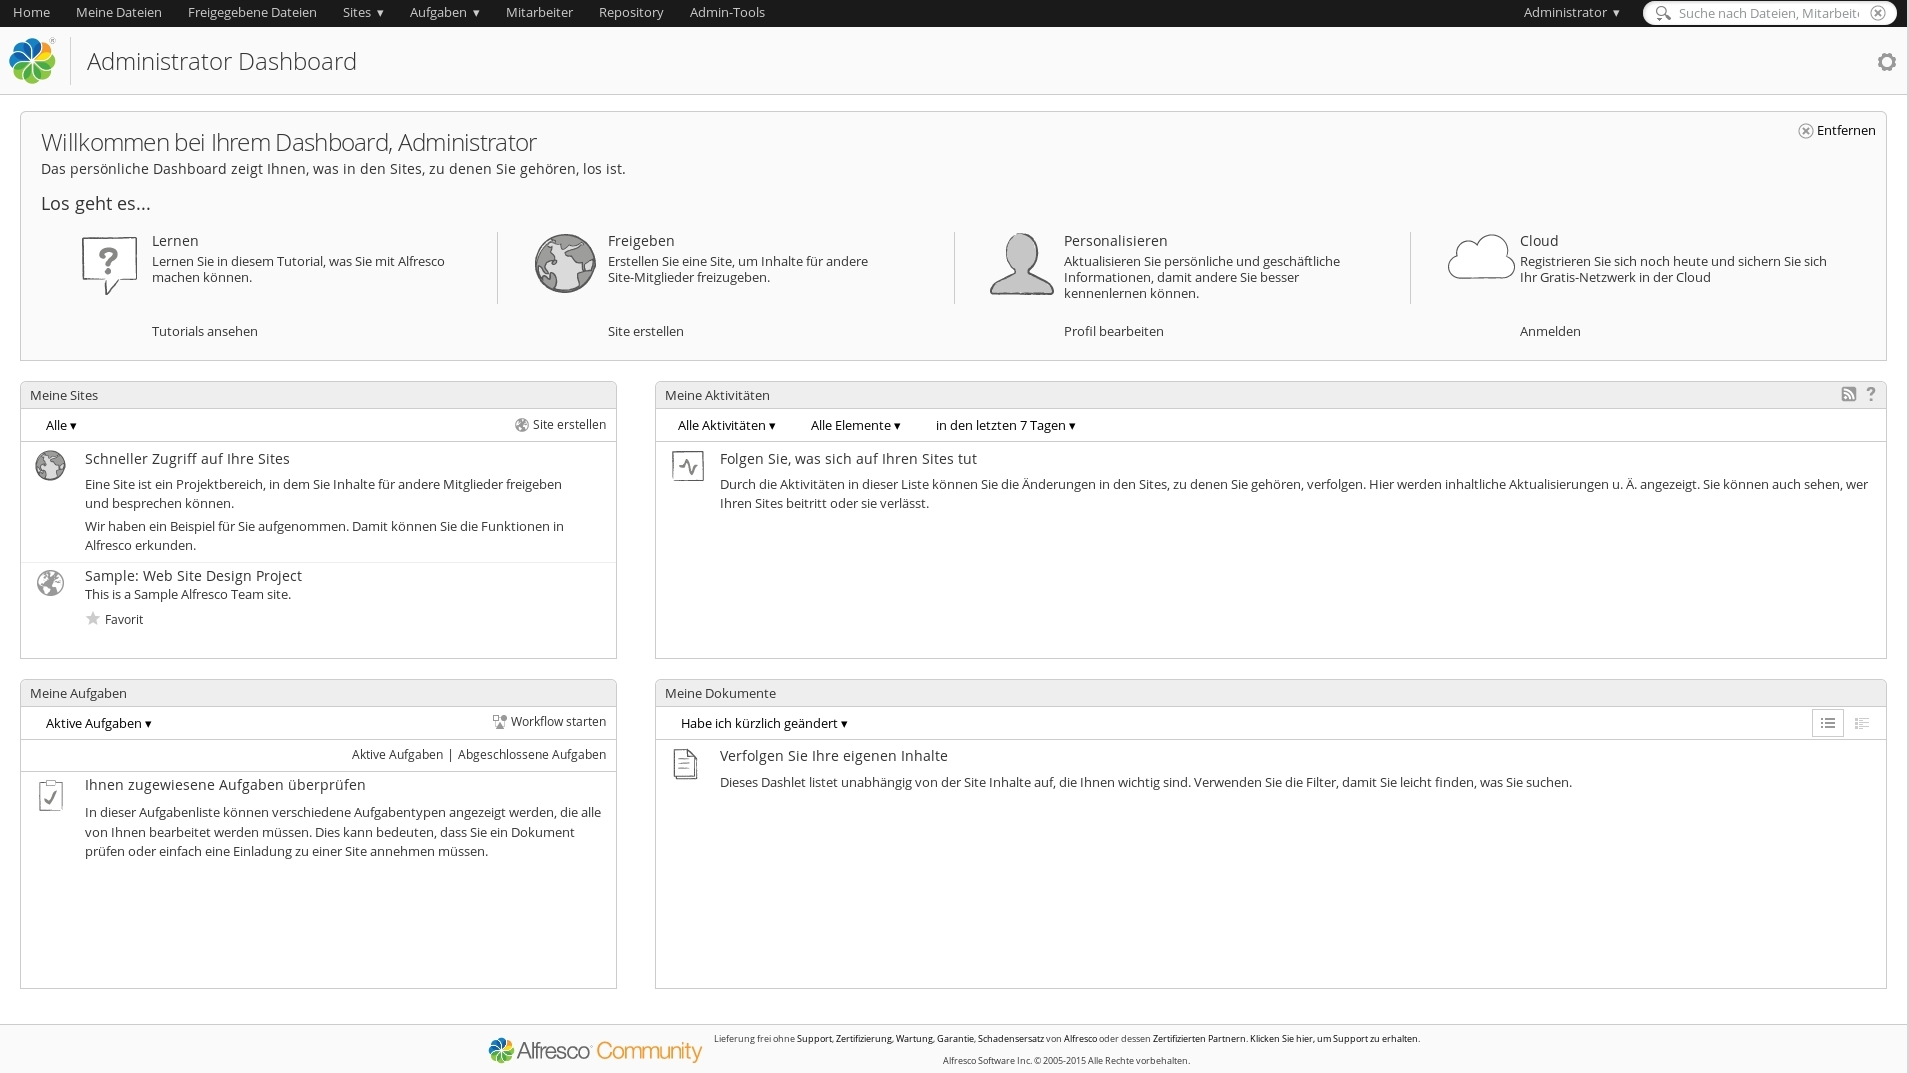
\includegraphics[width=16cm]{Bilder/Alfresco_Oberflaeche.jpg}
\caption{"`Administrator Dashboard"' von Alfresco}
\label{Alfresco Dashboard}
\centering
\end{figure}

Wird eine Datei in Alfresco eingef\"ugt, was per Drag \& Drop geht, werden automatisch schon vorhandene Metadaten aus der Datei herausgelesen. Hierbei werden zum Beispiel bei Bildern auch \ac{Exif}-Daten gelesen und angezeigt, wie in der Abbildung im Anhang \ref{Exif-Metadaten von Alfresco} zu sehen ist. 

Durch die "`Sites"', welche Alfresco bietet ist es ganz leicht m\"oglich, f\"ur alle bestehenden Systeme der \ac{LUBW} eine eigene "`Site"' zu erstellen. Da Alfresco f\"ur jedes Dokument eine Eindeutige ID vergibt, ist es sogar m\"oglich Dokumente von verschiedenen Seiten zu verlinken.
\cite{Eval_DMS_Bachelor}

Die Vorraussetzung, das neue Metadaten hinzugef\"ugt werden, und diese Gruppiert werden k\"onnen ist in Alfresco gegeben. Dies wird \"uber XML-Definitionen erledigt, welche dann unter Alfresco genutzt und in Workflows eingebaut werden k\"onnen. \cite{Alfresco_Custom_Content_Types} \cite{Professional_Alfresco}

Alfresco bietet die M\"oglichkeit durch viele verschiedene Schnittstellen eine breite Auswahl wie ein Frontend angebunden werden kann. Eine Anbindung kann zum Beispiel \"uber \ac{REST}, \"uber WebDAV oder \"uber die "`Alfresco One \ac{API}"' erfolgen. \cite{Alfrsco_Doku}

Auch eine Versionierung von Dokumenten ist m\"oglich, wobei eine neue Version die alte nicht einfach ersetzt. Alte Versionen k\"onnen auch weiterhin eingesehen werden.

Da Alfresco Open Source ist, ist es nicht nur kostenlos, sondern kann auch mit eigenen Tools erweitert werden. Dies kann zum einen \"uber direkte Programmierung im Quellcode geschehen oder zum anderen \"uber Aspekte, da Alfresco Aspektorientiert programmiert ist. \cite{Alfresco_und_Liferay}

\subsection{Open Xchange}

\subsection{Auswertung der M\"oglichkeiten}\label{Auswertung ECM}
\textcolor{green}{\checkmark} \textcolor{red}{X} \textcolor{orange}{\checkmark X}

\begin{table}[htbp]
\begin{center}
\begin{tabular}{|c|c|c|c|}
\hline
Anforderung: & agorum core & Alfresco & Open Xchange\\ \hline
 Metadatenstandards Implementiert & \textcolor{green}{\checkmark} 	& \textcolor{green}{\checkmark}		& \\ \hline
 Mehrere Systeme in einem & \textcolor{green}{\checkmark} 		& \textcolor{green}{\checkmark}		& \\ \hline
 Gliederung von Metadaten & \textcolor{orange}{\checkmark X} 		& \textcolor{green}{\checkmark}		& \\ \hline
 Vierschiedene Schnittstellen & \textcolor{green}{\checkmark} 		& \textcolor{green}{\checkmark}		& \\ \hline
 Versionierbarkeit von Dokumenten & \textcolor{orange}{\checkmark X} 	& \textcolor{green}{\checkmark}		& \\ \hline
 Kostenfreie Nutzung & \textcolor{orange}{\checkmark X} 		& \textcolor{green}{\checkmark}		& \\ \hline
\end{tabular}
\end{center}
\caption{Mapping der Bildarchiv Attribute}
\label{Systemvergleich}
\end{table}